\chapter{Theoretical Background}

% In your case, it could for instance contain the math of camera models, the theory of feature point detection and matching, motion field models, in your case in particular the model of a moving plane, parameterization of motion in terms of rotation matrices and translation vectors, and how they are computed from a set of feature point correspondences 

\section{Keypoint detection}

\subsection{What are keypoints}
According to Trucco \& Verri (1998) \cite{book} a local keypoint is defined as a local, meaningful, detectable part of an image. In the following, the term keypoint will be used for local keypoint. A keypoint is a local feature of an image, a part with some properties that differentiates it from other parts of the image. By meaningful, they mean that the feature is associated to interesting scene elements such as sharp intensity variations created by the contours of the objects in the scene. To be detectable they state that location algorithms must exist, if not, a keypoint would be of no use.

\subsection{Keypoint Detection}
There is a wide variety of keypoint detectors, each with their own way of finding keypoints. The two big categories they can be divided in are corner detectors and scale-space detectors. Examples of corner detectors are Harris, FAST and Shi-Tomasi. SIFT and SURF are examples of scale-space detectors. The advantage of corner detectors is that they are quite invariant to view changes. On the other hand, scale changes pose a problem. Scale-space detectors on the other hand try to detect keypoints on different scales of the image to find scale invariant keypoints

\subsection{Keypoint Description}
The detection of keypoints is not enough. If we want to work with them, we need a way to describe them. Otherwise, there is not way of knowing which keypoint in one image corresponds with which keypoint in another image. To do this, we need keypoint descriptors. Once again, there are lots of different keypoint descriptors that can be divided in continuous and binary keypoint descriptors. A continuous keypoint descriptor is nothing more than a high-dimensional real-valued vector describing the surroundings of the keypoint. While a binary keypoint descriptor is an vector of bits. The use of bits has the advantage that Hamming distance can be used to compare descriptors, which is very efficient. Also, storing binary values is cheaper than real values (using floating point).

An important feature of keypoint descriptors is their robustness, SIFT and SURF (continuous descriptors) for instance are robust to illumination, rotation and scale changes. BRIEF (binary descriptor) on the other hand is only robust to illumination, so illumination and scale changes are a problem when using BRIEF. ORB (binary descriptor) tried to eliminate this shortcoming of BRIEF and is invariant to illumination and rotation.

\section{Oriented FAST and rotated BRIEF (ORB)}
ORB is based on a combination of the FAST keypoint detector and the BRIEF keypoint descriptor. With ORB, Rublee et al. (2011) \cite{6126544} didn't just develop a combination of FAST and BRIEF, but enhanced it with extra features to make it rotation invariant and resistant to noise while maintaining the focus on speed.

\subsection{FAST Keypoint Orientation (oFAST)}
Features from Accelerated Segment Test or FAST, proposed by Rosten \& Drummond \cite{10.1007/11744023_34} is a keypoint detector developed with real-time applications in mind. It has thus, as the name suggest, good speed performance. However, the problem with FAST is that there is no orientation component. This is the first thing added by Rublee et al. (2011) \cite{6126544}.\bigskip

\subsubsection{Features from Accelerated Segment Test (FAST)}
To detect if pixel $p$ is a corner, the pixels on circle with radius $r$ around $p$ are considered, see Figure \ref{fig:fastcircle}. In ORB, $r$ equals 9, which is called FAST-9. The intensity of $p$ is $I_p$. To decide if $p$ is a corner, FAST uses a threshold value $t$. If there exists a set of $n$ (usually 12) contiguous pixels on the circle that are either all brighter than $I_p + t$ or all darker than $I_p - t$, then $p$ is considered a corner.\bigskip

\begin{figure}
    \centering
    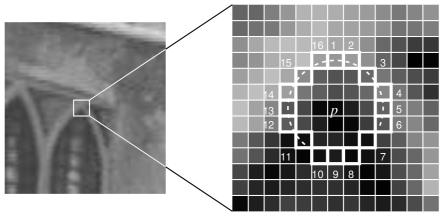
\includegraphics[width=1\textwidth]{figures/fast_circle.jpg}
    \caption{Fast with radius 3}
    \captionsource{Source: }{\cite{10.1007/11744023_34}}
    \label{fig:fastcircle}
\end{figure}

To make this process even faster, a high-speed test was introduced to eliminate a large number of non-corners. This high-speed test checks only four pixels, the ones on top, bottom, left and right. In Figure \ref{fig:fastcircle} these are pixels 1, 5, 9 and 13. At least three out of four of these pixels have to be either all brighter than $I_p + t$ or all darker than $I_p - t$. If this is not the case, there is no possibility for $p$ to be a corner. If this is the case, the full test will decide whether the $p$ is a corner.\bigskip

The problem with FAST is that it doesn't produce a value to indicate how much of a corner a certain pixel is. To cope with this shortcoming, ORB uses a Harris corner measure \cite{Harris1988ACC} to sort the keypoints detected by the FAST detector. After using FAST with a low threshold value (to ensure at least $N$ keypoints), it sorts the corners based on the Harris measure, leaving only the top $N$ points. As FAST doesn't produce multi-scale features, a scale pyramid is used to calculate FAST features at each level in the pyramid.

\subsubsection{Orientation using Intensity Centroid}
ORB uses Intensity Centroid \cite{ROSIN1999291}, a measure of corner orientation. It uses geometric moments to determine the corner orientation. Rosin defines the momentum as: 
\begin{equation}
    m_{pq} = \sum_{x,y} x^p y^q I(x, y),
\end{equation}
the centroid can then be found by:
\begin{equation}
    C = (\frac{m_{10}}{m_{00}},\frac{m_{01}}{m_{00}}).
\end{equation}
Placing $O$ at the center of the corner, a vector $\Vec{OC}$ can be created, the corner orientation is then:
\begin{equation}
    \theta = atan2(m_{01}, m_{10})
\end{equation}
where atan2(x, y) or 2-argument arctangent is defined as the angle in the Euclidean plane, given in radians, between the positive x axis and the ray to the point $(x, y) \neq (0, 0)$ \cite{unknown-author-2022}.\bigskip

ORB improves the rotation invariance even more by making sure that the moments are computed with $x$ and $y$ remaining within a circular region of radius $r$. \cite{6126544} found the patch size to be a fit value for $r$. This means $x$ and $y$ run from $[-r, r]$. $\mid C\mid$ approaching 0 makes the measure become unstable, but this is rarely the case for FAST corners \cite{6126544}.

\subsection{Rotation-Aware BRIEF (rBRIEF)}
We now have keypoints and their orientation, the next step is to compute the descriptor using BRIEF. As stated before, BRIEF is not invariant to rotation, which is why ORB introduced a modification: Rotation-Aware BRIEF.

\subsubsection{Binary Robust Independent Elementary Features (BRIEF)}
BRIEF \cite{10.1007/978-3-642-15561-1_56} uses a small number of pairwise comparisons to classify patches from which it makes a bit vector. They defined the test $\tau$ on patch $\boldsymbol{p}$ like this:
\begin{equation}
    \tau(\boldsymbol{p};\boldsymbol{x},\boldsymbol{y}) := \left\{\begin{array}{ll}
         1\quad : \boldsymbol{p}(\boldsymbol{x}) < \boldsymbol{p}(\boldsymbol{y})\\
         0\quad : \boldsymbol{p}(\boldsymbol{x}) \geq \boldsymbol{p}(\boldsymbol{y})
    \end{array} \right.,
\end{equation}
with $\boldsymbol{p}(\boldsymbol{x})$ the pixel intensity in a smoothed version of $\boldsymbol{p}$ at $\boldsymbol{x} = (u, v)^T$. The BRIEF descriptor is then defined as the $n$-dimensional bitstring
\begin{equation}
    f_n(\boldsymbol{p}) := \sum_{1\leq i\leq n} 2^{i-1}\tau(\boldsymbol{p};\boldsymbol{x},\boldsymbol{y}) .
\end{equation}

Relying on the experiments of \cite{10.1007/978-3-642-15561-1_56}, ORB will use $n = 256$, a Gaussian distribution around the center of the patch and smooth the image using an integral image where each test point is a $5 \times 5$ subwindow of a $31 \times 31$ pixel patch. Based on experimental results in \cite{10.1007/978-3-642-15561-1_56} and their own these showed to be performing well.

\subsubsection{Steered BRIEF}
As stated before, BRIEF is not robust when it comes to in-plane rotations. Even small rotations over a few degrees drops the amount of inliers significantly \cite{6126544}. ORB tackles this problem by introducing Steered BRIEF which steers the BRIEF descriptor according to the orientation of the keypoint. \bigskip

To get to the steered BRIEF operator, a $2\times n$ matrix is defined as follows:
\begin{equation}
    S = \begin{pmatrix}
    x_1,...,x_n \\
    y_1,...,y_n
    \end{pmatrix}
\end{equation}

The steered version $S_\theta$ of $S$ is constructed using the rotation matrix $R_\theta$, $\theta$ being the orientation of the patch:
\begin{equation}
    S_\theta = R_\theta S
\end{equation}
The steered BRIEF operator is now
\begin{equation}
    g_n(\boldsymbol{p},\theta):=f_n(\boldsymbol{p})\mid(x_i,y_i)\in S_\theta
\end{equation}

A lookup table is constructed for values of $\theta = 2k\pi/30, k \in \mathbb{N}_0$. If the keypoint orientation $\theta$ is consistent across views, the correct set of points $S_\theta$ will be used to compute the descriptor.

\subsubsection{rBRIEF}
However, the benefit of rotational invariance comes at a price. \cite{6126544} noticed a loss of variance and high correlation among the binary tests. To cope with these shortcomings, they developed a learning method to choose a good subset of binary tests. The goal is to have high variance and means close to 0.5, as well as being uncorrelated. To do this, they look at all binary tests.\bigskip

\cite{6126544} proposes the following greedy algorithm to get a set of uncorrelated tests with a mean close to 0.5:
\begin{enumerate}
    \item Run each test  against all training patches.\smallskip
    \item Order the tests by their distance from a mean of 0.5, forming the vector T.\smallskip
    \item Greedy search:\smallskip
    \begin{enumerate}
        \item Put the first test into the result vector R and remove it from T.\smallskip
        \item Take the next test from T, and compare it against all tests in R. If its absolute correlation is greater than a threshold, discard it; else add it to R.\smallskip
        \item Repeat the previous step until there are 256 tests in R. If there are fewer than 256, raise the threshold and try again.\smallskip
    \end{enumerate}
\end{enumerate}

They showed that this is a good method to ensure high diversity and low correlation.\bigskip

Rublee et al.\cite{6126544} is the perfect paper for a more detailed explanation of ORB, along with an evaluation and comparison with SURF and SIFT. 

% \section{Visual Odometry}
% Visual Odometry (VO) is a process that calculates the motion (rotation and translation) of a body based on the images of a single or multiple cameras attached to the body. There are multiple ways to achieve this. 

\section{Motion estimation}
Now that keypoints are detected and matched, the relation between these keypoints can be expressed as a Homography. The Homography is the transformation between the planes in the respective frames. Suppose we have keypoint $\boldsymbol{X} = [X_1, X_2, X_3]^T$ that has been matched to keypoint $\boldsymbol{X'} = [X_1', X_2', X_3']^T$. The movement of this keypoint can be described as follows: 

\begin{equation} \label{eq:1}
    \begin{pmatrix}
        X_1' \\
        X_2' \\
        X_3'
    \end{pmatrix}
    = \boldsymbol{R}
    \begin{pmatrix}
        X_1 \\
        X_2 \\
        X_3
    \end{pmatrix}
    + \boldsymbol{T}
\end{equation}
where $\boldsymbol{R}$ is a $3 \times 3$ matrix describing the rotation and $\boldsymbol{T}$ a vector describing the translation. Also valid is this: 
\begin{equation}
    \begin{pmatrix}
        X_1' \\
        X_2' \\
        X_3'
    \end{pmatrix}
    = \boldsymbol{H}
    \begin{pmatrix}
        X_1 \\
        X_2 \\
        X_3
    \end{pmatrix}.
\end{equation} 

So it is clear that there is a relation between \boldsymbol{H} on the one hand and $\boldsymbol{R}$ and $\boldsymbol{T}$ on the other hand.\bigskip

\subsection{Essential matrix}
OpenCV has a method \textit{findHomography} to find this Homography based on the keypoints detected and matched. We need to use this homography to compute rotation-matrix $\boldsymbol{R}$ and translation-vector $\boldsymbol{T}$. In \cite{improc} T. S. Huang proposed that with at least eight keypoint matches a two-step linear algorithm can be developed. To do this, intermediate values called essential parameters need to be estimated first. These essential parameters form a matrix $\boldsymbol{E}$ called the essential matrix:
\begin{equation}
    \boldsymbol{E} = 
    \begin{pmatrix}
        e_1&e_2&e_3 \\
        e_4&e_5&e_6 \\
        e_7&e_8&e_9 
    \end{pmatrix}
    = \begin{pmatrix}
        0&-T_3&T_2 \\
        T_3&0&-T_1 \\
        -T_2&T_1&0
    \end{pmatrix}
     \boldsymbol{R}
\end{equation}

These nine essential elements are not all independent due to the fact that  $\boldsymbol{E}$ is a product of a skew-symmetric matrix and a rotation matrix.\bigskip

\cite{tekalp} states that vectors $\boldsymbol{X'}$, $\boldsymbol{T}$ and $\boldsymbol{RX}$ are coplanar, since $\boldsymbol{X'} = \boldsymbol{RX} + \boldsymbol{T}$ from (\ref{eq:1}). So now we have 
\begin{equation}
    \boldsymbol{X} \cdot (\boldsymbol{T} \times \boldsymbol{RX}) = 0
\end{equation}
because $(\boldsymbol{T} \times \boldsymbol{RX}$ is orthogonal to this plane. From this, it follows that 
\begin{equation} \label{eq:2}
    \boldsymbol{X'^TEX} = 0
\end{equation}

We want to obtain a relationship in terms of the image plane coordinates. To do this, we divide both sides of \ref{eq:2} by $X_3 X'_3$:
\begin{equation} \label{eq:essential}
    \begin{pmatrix}
        x_1'&x_2&1
    \end{pmatrix}
    \boldsymbol{E}
    \begin{pmatrix}
        x1 \\
        x2 \\
        1
    \end{pmatrix}
    = 0
\end{equation}

This linear homogeneous equation, in terms of the nine essential parameters, has either no solution or infinitely many solutions. By setting one of these nine essential parameters to one in the equation above, we can solve it for the remaining eight essential parameters. The essential parameter set to one is used as a scale factor. It's important to note that because of scale ambiguity in perspective projection, translation can only be estimated up to a scale factor.

\subsection{Estimation of the Essential Parameters}
To estimate these essential parameters, \cite{tekalp} proposes three methods: a linear lest squares method, an optimisation method requiring at least eight keypoint matches and a nonlinear method where only five, six or seven keypoint matches are needed. We'll discuss the Linear Least Squares Method.\bigskip

As stated before, one of the essential parameters will be set to one. Take $e_9 = 1$, then equation (\ref{eq:essential}) can be written as:
\begin{equation}
    \begin{pmatrix}
        x_1'x_1 &
        x_1'x_2 &
        x_1' &
        x_2'x_1 &
        x_2'x_2 &
        x_2' &
        x_1 &
        x_2
    \end{pmatrix}
    \begin{pmatrix}
        e1 \\
        e2 \\
        e3 \\
        e4 \\
        e5 \\
        e6 \\
        e7 \\
        e8 \\
    \end{pmatrix}
    = -1
\end{equation}

This linear equation in eight essential parameters can be set up as a system of $N$ linear equations in 8 unknowns. To solve this, we need at least $N \geq 8$ keypoint matches. The solution of this equation gives the essential matrix $\boldsymbol{E}$ up to a scale factor (as discussed before). We took $e_9$ as the scale factor, but all of the other essential parameters could have been chosen as well. When using this method, $e_i, i = 1,...,9$ will be chosen based on the condition number, the $e_i$ that yields the smallest condition number will be chosen as scale factor.

To have a solution for this equation, the coefficient matrix needs to have full rank, \cite{tekalp} states that this is the case if $\boldsymbol{T} \neq 0$ and the shape of the 3-D surface satisfies certain conditions, called the surface constraint.

Other methods to estimate the essential parameters can be found in \cite{tekalp}.

\subsection{Decomposition of the Essential Matrix}
Now that we have the essential parameters that make up the essential matrix $\boldsymbol{E}$, we can use this to compute rotation matrix $\boldsymbol{R}$ and translation vector $\boldsymbol{T}$.